Masterthesis: \cite{cdeutsch-master}

RNN Tau-ID PubNote: \cite{ATL-PHYS-PUB-2019-033}

RNNIP: \cite{ATL-PHYS-PUB-2017-003}

Things I have to explain:
\begin{itemize}
\item Features of hadronic \tauhad decays and how they compare to \tauhad faked by jets
\item BDT approach and input variables
\item Training setup, i.e.\ samples (dijet \& $\gamma^*$)
\item Keras Tensorflow lwtnn \cite{lwtnn,keras,tensorflow2015-whitepaper,lstm}
\item Input variables
\item Reweighting of (fake) \tauhad \pT
\item Working point extraction
\item Tau lepton triggers in 2018 \cite{ATL-DAQ-PUB-2019-001}
\end{itemize}



\begin{figure}[htbp]
  \centering

  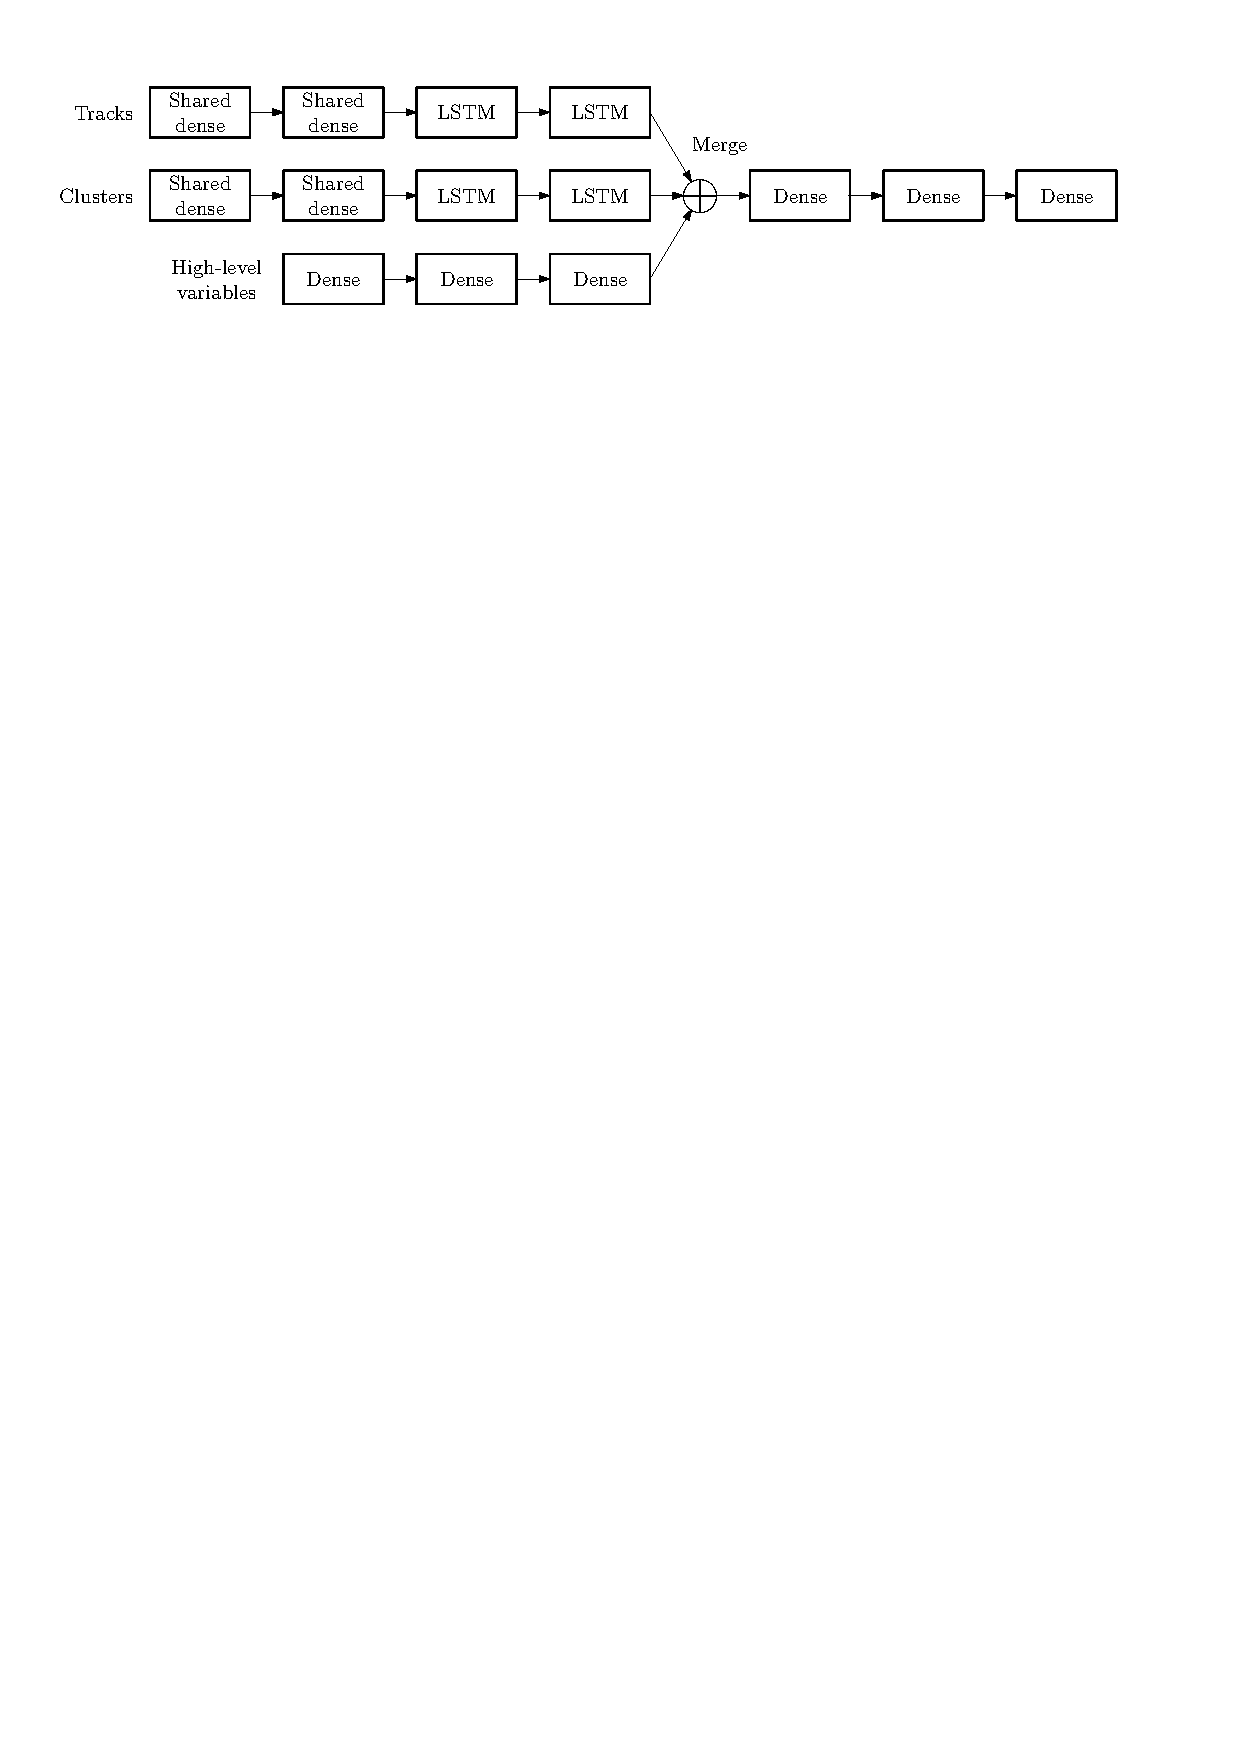
\includegraphics[width=0.9\textwidth]{tauid/pubnote/rnn_network_architecture}

  \caption{Network Architecture of the RNN \tauhad-identification
    algorithm \cite{ATL-PHYS-PUB-2019-033}}
  \label{fig:tauid_network_architecture}
\end{figure}


\begin{figure}[htbp]
  \centering

  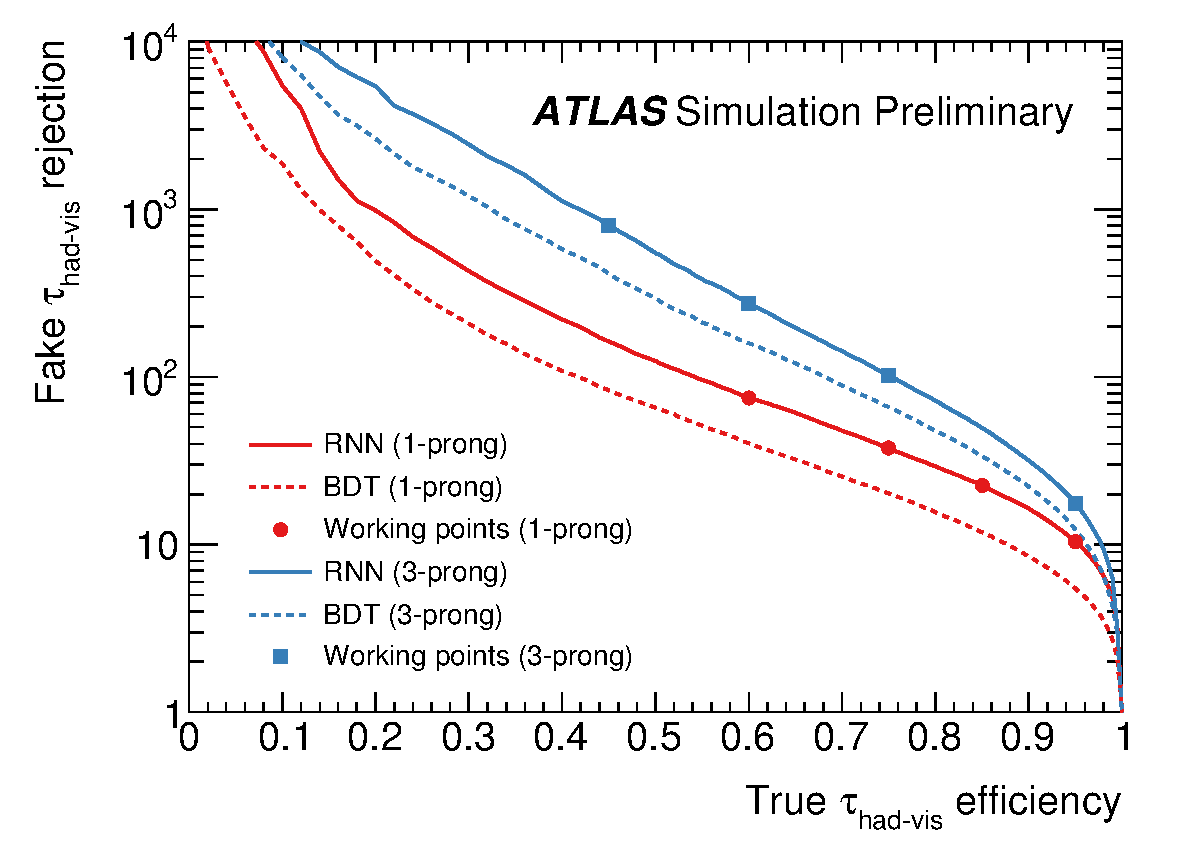
\includegraphics[width=0.5\textwidth]{tauid/pubnote/rnn_bdt_roc}

  \caption{Receiver operating characteristic of the RNN
    \tauhad-identification algorithm \cite{ATL-PHYS-PUB-2019-033}}
  \label{fig:tauid_rnn_bdt_roc_comparison}
\end{figure}

\begin{table}
  \centering

  \begin{tabular}{lcccccc}
    \toprule
                  & \multicolumn{2}{c}{Signal efficiency} & \multicolumn{2}{c}{Background rejection (BDT)} & \multicolumn{2}{c}{Background rejection (RNN)} \\
    Working point  & 1-prong & 3-prong & 1-prong & 3-prong & 1-prong & 3-prong \\
    \midrule
    Tight          & 60\%    & 45\%    & 40      & 400  & 70   & 700 \\
    Medium         & 75\%    & 60\%    & 20      & 150  & 35   & 240 \\
    Loose          & 85\%    & 75\%    & 12      & 61   & 21   & 90  \\
    Very loose     & 95\%    & 95\%    & 5.3     & 11.2 & 9.9  & 16  \\
    \bottomrule
  \end{tabular}
  \todo[inline]{This text is stolen from the PUB note}
  \caption{List of defined working points with fixed true \tauhadvis
    selection efficiencies and the corresponding background rejection
    factors for misidentified \tauhadvis in dijet events for the BDT
    and RNN classifiers. Adapted from~\cite{ATL-PHYS-PUB-2019-033}.}
  \label{tab:rnn_wps}
\end{table}

%%% Local Variables:
%%% mode: latex
%%% TeX-master: "../../phd_thesis"
%%% End:
